%%%%%%%%%%%%%%%%%%%%%%%%%%%%%%%%%%%%%%%%%%%%%%%%%%%%%%
% A Beamer template for University of Wollongong     %
% Based on THU beamer theme                          %
% Author: Qiuyu Lu                                   %
% Date: July 2024                                    %
% LPPL Licensed.                                     %
%%%%%%%%%%%%%%%%%%%%%%%%%%%%%%%%%%%%%%%%%%%%%%%%%%%%%%

\documentclass[aspectratio=169]{beamer}
\usepackage[scaled=0.9]{helvet}
\usepackage{courier}
\usepackage[T1]{fontenc}
\usepackage{hyperref}
\usepackage{latexsym,amsmath,xcolor,multicol,booktabs,calligra}
\usepackage{graphicx,pstricks,listings,stackengine}


\usepackage{inputenx} 
\usetheme{Madrid}
\usecolortheme{seahorse}

\usepackage{tikz}
% Configuration de TikZ pour la mise en évidence
\tikzset{
    highlight on/.style={
        alt={#1{fill=red!80!black, color=red!80!black}{fill=gray!30!white, color=gray!30!white}},
    },
}

\author{EL HASSANI Nabil}
\title{Design pattern}
\subtitle{Introduction aux design patterns}
\institute{
    Efrei \\
    Université Paris Panthéon-Assas
    }
    \date{\small \today}
\usepackage{UoWstyle}

% defs
\def\cmd#1{\texttt{\color{red}\footnotesize $\backslash$#1}}
\def\env#1{\texttt{\color{blue}\footnotesize #1}}
\definecolor{deepblue}{rgb}{0,0,0.5}
\definecolor{deepred}{RGB}{153,0,0}
\definecolor{deepgreen}{rgb}{0,0.5,0}
\definecolor{halfgray}{gray}{0.55}

\lstset{
    basicstyle=\ttfamily\small,
    keywordstyle=\bfseries\color{deepblue},
    emphstyle=\ttfamily\color{deepred},    % Custom highlighting style
    stringstyle=\color{deepgreen},
    numbers=left,
    numberstyle=\small\color{halfgray},
    rulesepcolor=\color{red!20!green!20!blue!20},
    frame=shadowbox,
}

%\setbeameroption{show notes on second screen=left}
\titlegraphic{
\includegraphics[height=1.5cm]{pic/efrei_logo.png}}
%==========================================================
\begin{document}
%==========================================================
% Page de titre
\begin{frame}
    \titlepage
\end{frame}

% Plan de la présentation
\begin{frame}
    \frametitle{Plan de la Présentation}
    \tableofcontents[hideallsubsections]
\end{frame}

%==========================================================
\section{Introduction}

\subsection{Objectifs du Cours}

\begin{frame}{Objectifs du Cours}
    \begin{itemize}
        \item \textbf{Comprendre} les concepts fondamentaux des \textbf{Design Patterns} en POO.
        \item \textbf{Acquérir} les compétences pour \textbf{identifier} et \textbf{appliquer} les patterns appropriés en fonction des problèmes rencontrés.
        \item \textbf{Développer} la capacité à concevoir des logiciels \textbf{flexibles}, \textbf{réutilisables} et \textbf{maintenables}.
        \item \textbf{Maîtriser} les patterns les plus courants tels que \textbf{Singleton}, \textbf{Factory}, \textbf{Adapter}, \textbf{Observer}, \textbf{Strategy}.
    \end{itemize}
\end{frame}

\subsection{Plan du Cours}

\begin{frame}{Plan du Cours}
    \tableofcontents
\end{frame}

\subsection{Pourquoi les Design Patterns ?}

\begin{frame}{Pourquoi étudier les Design Patterns ?}
    \begin{itemize}
        \item \textbf{Réutilisation} de solutions éprouvées.
        \item \textbf{Amélioration} de la communication entre développeurs.
        \item \textbf{Facilitation} de la maintenabilité et de l'évolution du code.
        \item \textbf{Renforcement} de la flexibilité et de la modularité des applications.
    \end{itemize}
\end{frame}

%==========================================================
\section{Historique des Design Patterns}
\begin{frame}{Origines des Design Patterns}
    \begin{columns}
        \begin{column}{0.6\textwidth}
            \begin{itemize}
                \item \textbf{Années 1970} : Introduction du concept de "patterns" par \textbf{Christopher Alexander}, architecte.
                \item \textbf{Application en informatique} : Les idées d'Alexander sont adaptées au développement logiciel.
                \item \textbf{1994} : Publication du livre \textit{"Design Patterns: Elements of Reusable Object-Oriented Software"}.
            \end{itemize}
        \end{column}
        \begin{column}{0.4\textwidth}
            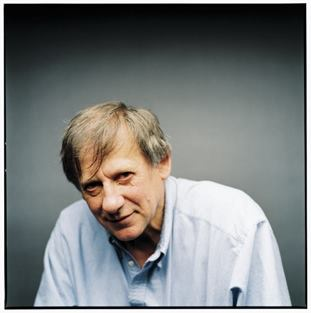
\includegraphics[width=0.8\textwidth]{pic/christopher_alexander.jpg}
            \begin{center}
                \small{\textit{Christopher Alexander}}
            \end{center}
        \end{column}
    \end{columns}
\end{frame}

  \begin{frame}{Le Gang of Four (GoF)}
    \begin{columns}
      \begin{column}{0.6\textwidth}
        \begin{itemize}
          \item \textbf{Erich Gamma}
          \item \textbf{Richard Helm}
          \item \textbf{Ralph Johnson}
          \item \textbf{John Vlissides}
        \end{itemize}
        \pause
        \begin{itemize}
          \item Leur livre a profondément influencé la conception logicielle.
          \item A établi un vocabulaire commun pour les développeurs.
          \item A favorisé la diffusion des bonnes pratiques en POO.
        \end{itemize}
      \end{column}
      \begin{column}{0.4\textwidth}
        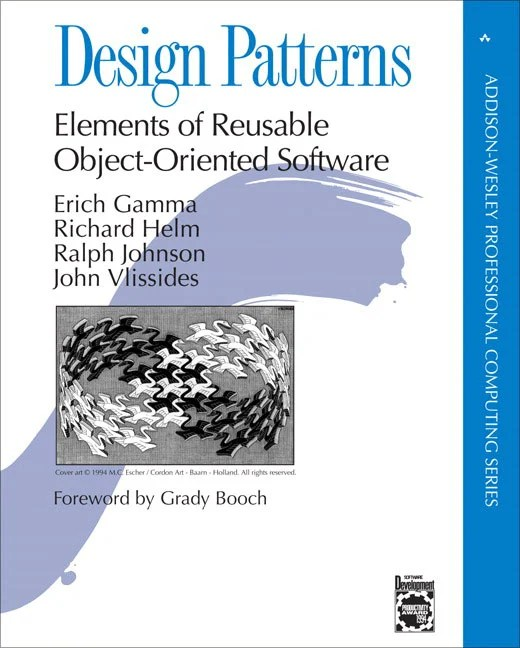
\includegraphics[width=0.9\textwidth]{pic/gof_book.jpg}
        \begin{center}
          \small{\textit{Couverture du livre du GoF}}
        \end{center}
      \end{column}
    \end{columns}
  \end{frame}

%==========================================================
\section{Pourquoi les Design Patterns ?}

\subsection{Des solutions réutilisables aux problèmes récurrents}

\begin{frame}{Des solutions réutilisables aux problèmes récurrents}
    \begin{columns}
        \begin{column}{0.6\textwidth}
            \begin{itemize}
                \item \textbf{Standardisation} des solutions pour des problèmes connus.
                \item \textbf{Gain de temps} : Évite de "réinventer la roue".
                \pause
                \item \textbf{Exemple} : Le \textbf{Singleton} pour garantir une seule instance d'une classe.
            \end{itemize}
        \end{column}
        \begin{column}{0.4\textwidth}
            \begin{center}
                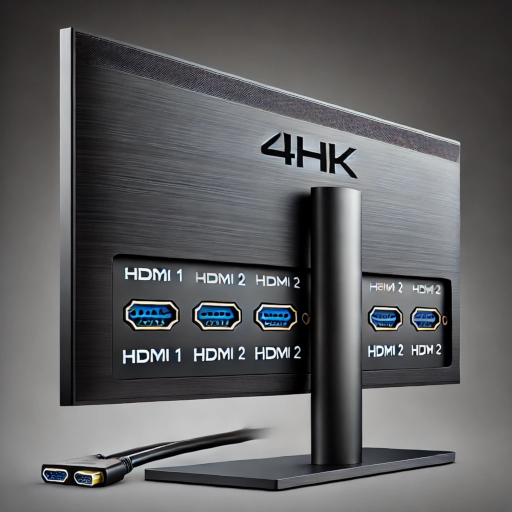
\includegraphics[width=0.8\textwidth]{pic/singleton_pattern.png}
            \end{center}
        \end{column}
    \end{columns}
\end{frame}

\subsection{Amélioration de la communication}

\begin{frame}{Amélioration de la communication}
    \begin{columns}
        \begin{column}{0.6\textwidth}
            \begin{itemize}
                \item \textbf{Vocabulaire commun} facilitant les échanges.
                \item \textbf{Clarté} dans la documentation et le code.
                \pause
                \item \textbf{Exemple} : "Utilisons un \textbf{Factory Method} ici."
            \end{itemize}
        \end{column}
        \begin{column}{0.4\textwidth}
            \begin{center}
                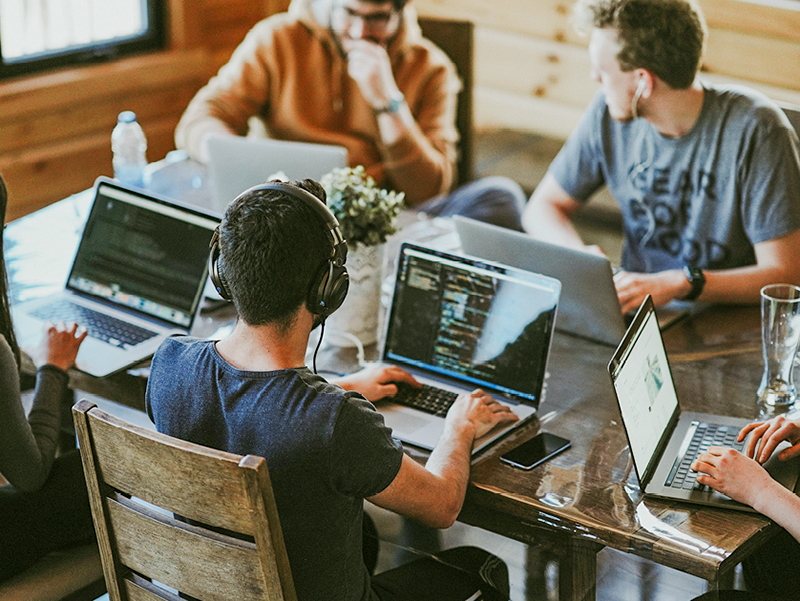
\includegraphics[width=0.8\textwidth]{pic/communication.png}
            \end{center}
        \end{column}
    \end{columns}
\end{frame}

\subsection{Facilitation de la maintenabilité et de l'évolution du code}
\begin{frame}{Facilitation de la maintenabilité et de l'évolution du code}
    \begin{columns}
        \begin{column}{0.6\textwidth}
            \begin{itemize}
                \item \textbf{Code modulaire} et \textbf{flexible}.
                \item \textbf{Facilité} d'ajout de nouvelles fonctionnalités.
                \pause
                \item \textbf{Exemple} : Le \textbf{Decorator} pour ajouter des responsabilités dynamiquement.
            \end{itemize}
        \end{column}
        \begin{column}{0.4\textwidth}
            \begin{center}
                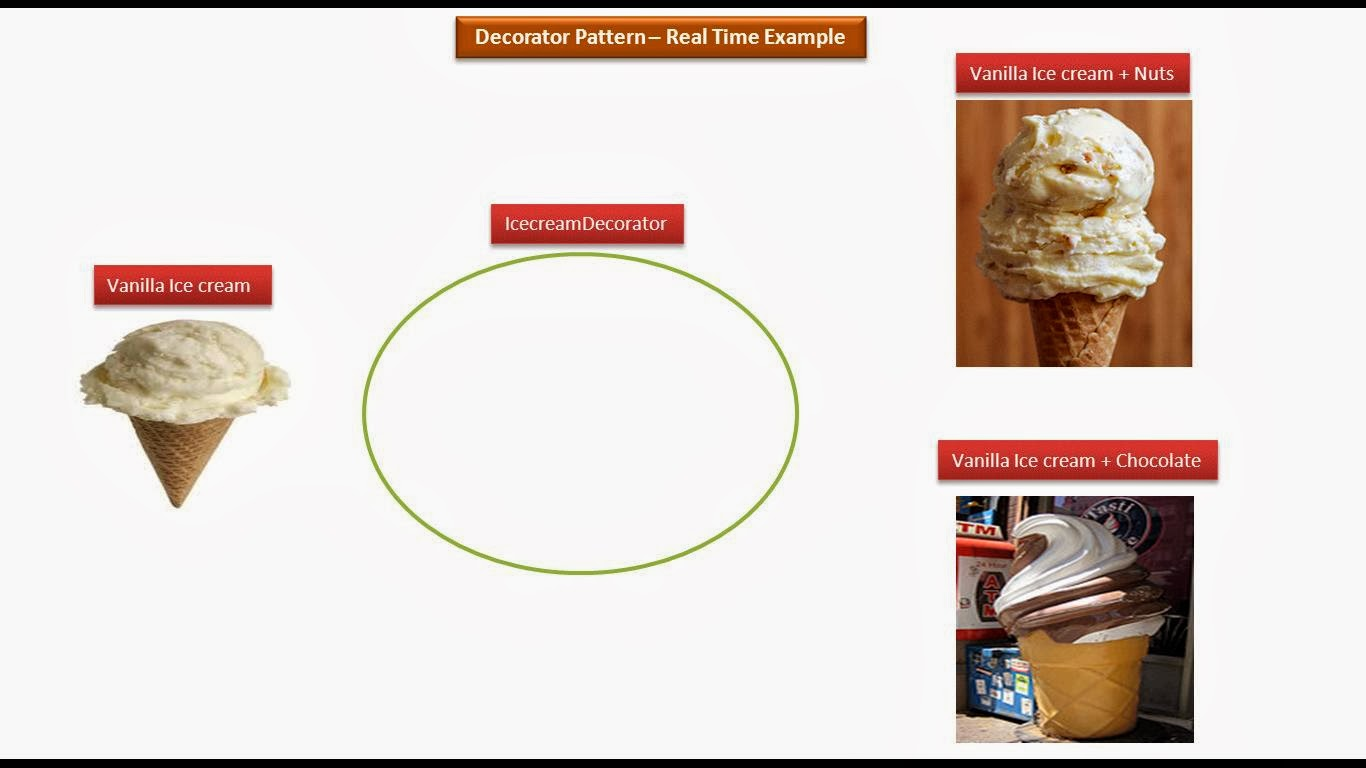
\includegraphics[width=1.0\textwidth]{pic/decorator_pattern.png}
            \end{center}
        \end{column}
    \end{columns}
\end{frame}
\subsection{Renforcement de la flexibilité et de la modularité}

\begin{frame}{Renforcement de la flexibilité et de la modularité}
    \begin{columns}
        \begin{column}{0.6\textwidth}
    \begin{itemize}
        \item \textbf{Séparation des préoccupations}.
        \item \textbf{Interopérabilité} entre les composants.
        \pause
        \item \textbf{Exemple} : Le \textbf{Adapter} pour faire collaborer des interfaces incompatibles.
    \end{itemize}
\end{column}
\begin{column}{0.4\textwidth}
    \begin{center}
        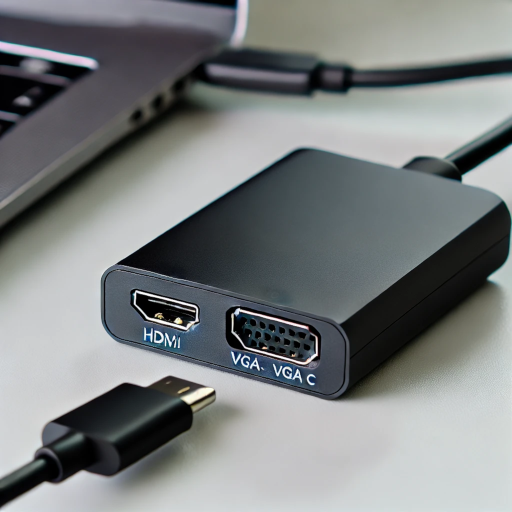
\includegraphics[width=0.8\textwidth]{pic/adapter_pattern.png}
    \end{center}
\end{column}
\end{columns}
\end{frame}

%==========================================================
\section{Catégories de Design Patterns}

\begin{frame}{Catégories de Design Patterns}
    \begin{columns}
        \begin{column}{0.6\textwidth}
            \begin{itemize}
                \item \textbf{Créationnels} : Gestion de la création des objets.
                    \begin{itemize}
                        \item \textbf{Exemples} : Singleton, Factory Method, Abstract Factory, Builder, Prototype.
                    \end{itemize}
                \item \textbf{Structurels} : Composition des classes et des objets.
                    \begin{itemize}
                        \item \textbf{Exemples} : Adapter, Decorator, Composite, Facade, Bridge, Proxy, Flyweight.
                    \end{itemize}
                \item \textbf{Comportementaux} : Interaction et responsabilité entre les objets.
                    \begin{itemize}
                        \item \textbf{Exemples} : Observer, Strategy, Command, Iterator, Mediator, State, Visitor, Template Method.
                    \end{itemize}
            \end{itemize}
        \end{column}
        \begin{column}{0.4\textwidth}
                \begin{center}
                    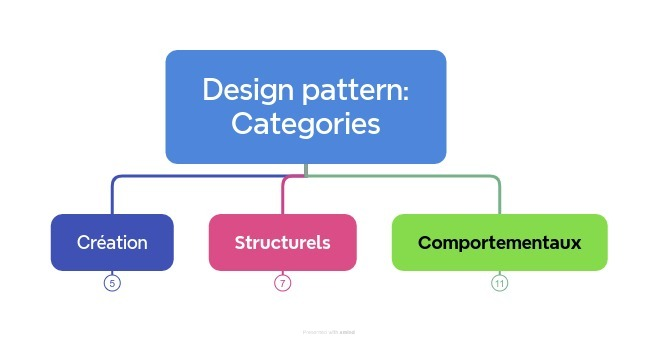
\includegraphics[width=1.0\textwidth]{pic/design_patterns_categories.jpg}
                \end{center}
            \end{column}
        \end{columns}
\end{frame}

\begin{frame}{Tableau Comparatif des Catégories}

\end{frame}

%==========================================================
\section{Rappel des Fondamentaux de la POO}

\subsection{Principes de la Programmation Orientée Objet}

\begin{frame}{Principes de la Programmation Orientée Objet}
    \begin{columns}
        \begin{column}{0.6\textwidth}
            \begin{itemize}
                \item \textbf{Encapsulation} : Regrouper les données et les méthodes.
                \item \textbf{Abstraction} : Cacher la complexité et ne montrer que l'essentiel.
                \item \textbf{Héritage} : Réutiliser le code en créant des sous-classes.
                \item \textbf{Polymorphisme} : Utiliser une interface commune pour des actions différentes.
            \end{itemize}
        \end{column}
        \begin{column}{0.4\textwidth}
            \pause
            \begin{center}
                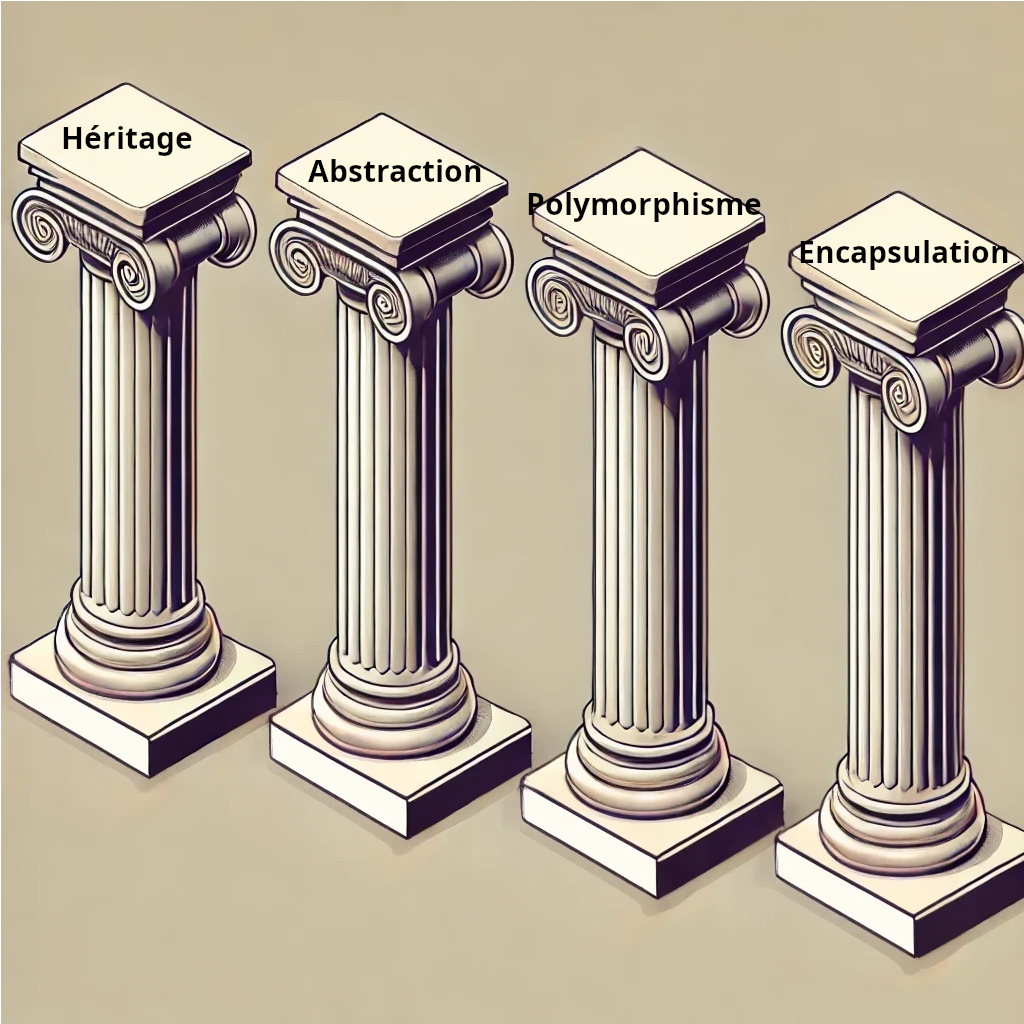
\includegraphics[width=0.6\textwidth]{pic/poo_principles.png}
            \end{center}
        \end{column}
    \end{columns}
\end{frame}

\subsection{Héritage vs Composition}

\begin{frame}{Comparaison : Héritage vs Composition}
    \begin{itemize}
        \item \textbf{Héritage} (\textit{est-un})
              \begin{itemize}
                  \item Avantages :
                        \begin{itemize}
                            \item Réutilisation du code.
                            \item Simplicité de conception.
                        \end{itemize}
                  \item Inconvénients :
                        \begin{itemize}
                            \item Couplage fort entre classes.
                            \item Rigidité face aux changements.
                        \end{itemize}
              \end{itemize}
        \item \textbf{Composition} (\textit{a-un})
              \begin{itemize}
                  \item Avantages :
                        \begin{itemize}
                            \item Flexibilité.
                            \item Faible couplage.
                        \end{itemize}
                  \item Inconvénients :
                        \begin{itemize}
                            \item Complexité initiale.
                            \item Plus de code à écrire.
                        \end{itemize}
              \end{itemize}
    \end{itemize}
\end{frame}

\begin{frame}{Recommandations}
    \begin{itemize}
        \item \textbf{Privilégier la composition} pour une meilleure flexibilité.
        \item \textbf{Utiliser l'héritage} lorsque les classes ont une relation naturelle de type \textit{est-un}.
        \item \textbf{Exemple UML} :
    \end{itemize}
    % \begin{center}
    %   \includegraphics[width=0.7\textwidth]{pic/uml_composition_inheritance.png}
    % \end{center}
\end{frame}

%==========================================================
\section{Études de Cas et Exemples}

\subsection{Exemple : Le Pattern Observer}

\begin{frame}{Exemple : Le Pattern Observer}
    \begin{itemize}
        \item \textbf{Problème} : Comment notifier automatiquement des objets lorsque l'état d'un autre objet change ?
        \item \textbf{Solution} : Utiliser le pattern \textbf{Observer} pour établir une relation entre un sujet et ses observateurs.
        \item \textbf{Cas d'utilisation} : Modèle-Vue-Contrôleur (MVC), événements GUI.
    \end{itemize}
    \pause
    % \begin{center}
    %   \includegraphics[width=0.7\textwidth]{pic/observer_pattern.png}
    % \end{center}
\end{frame}

\subsection{Exercice Pratique}

\begin{frame}{Exercice Pratique}
    \textbf{Scénario} : Vous développez une application de messagerie. Lorsqu'un nouvel utilisateur s'inscrit, tous les services associés (profil, notifications, emails) doivent être informés.

    \vspace{0.5cm}

    \textbf{Question} : Quel design pattern utiliseriez-vous pour implémenter cette fonctionnalité, et comment ?

    \vspace{0.5cm}

    \pause

    \textbf{Réponse attendue} : Utilisation du \textbf{Pattern Observer} pour que les services s'abonnent aux événements d'inscription.
\end{frame}

%==========================================================
\section{Ressources et Références}

\begin{frame}{Ressources et Références}
    \begin{itemize}
        \item \textbf{Livres} :
              \begin{itemize}
                  \item \textit{Design Patterns: Elements of Reusable Object-Oriented Software} - GoF
                  \item \textit{Head First Design Patterns} - Eric Freeman et al.
              \end{itemize}
        \item \textbf{Sites Web} :
              \begin{itemize}
                  \item \href{https://refactoring.guru/design-patterns}{Refactoring Guru}
                  \item \href{https://www.tutorialspoint.com/design_pattern/index.htm}{TutorialsPoint - Design Patterns}
              \end{itemize}
        \item \textbf{Communautés} :
              \begin{itemize}
                  \item \href{https://stackoverflow.com}{Stack Overflow}
                  \item \href{https://www.meetup.com/topics/softwaredev/}{Meetup - Software Development}
              \end{itemize}
    \end{itemize}
\end{frame}

%==========================================================
\begin{frame}{Questions ?}
    \begin{center}
        {\Huge\calligra Merci !}

        \vspace{1cm}

        \Large{Des questions ou des commentaires ?}

        \vspace{0.5cm}

        \small{Vous pouvez me contacter à : \href{mailto:votre.email@efrei.fr}{votre.email@efrei.fr}}
    \end{center}
\end{frame}

\end{document}